\documentclass[border=10pt]{standalone}
\usepackage{tikz}
\usetikzlibrary{shadows}
\usepackage{amsmath}
\usepackage{amssymb}

\begin{document}

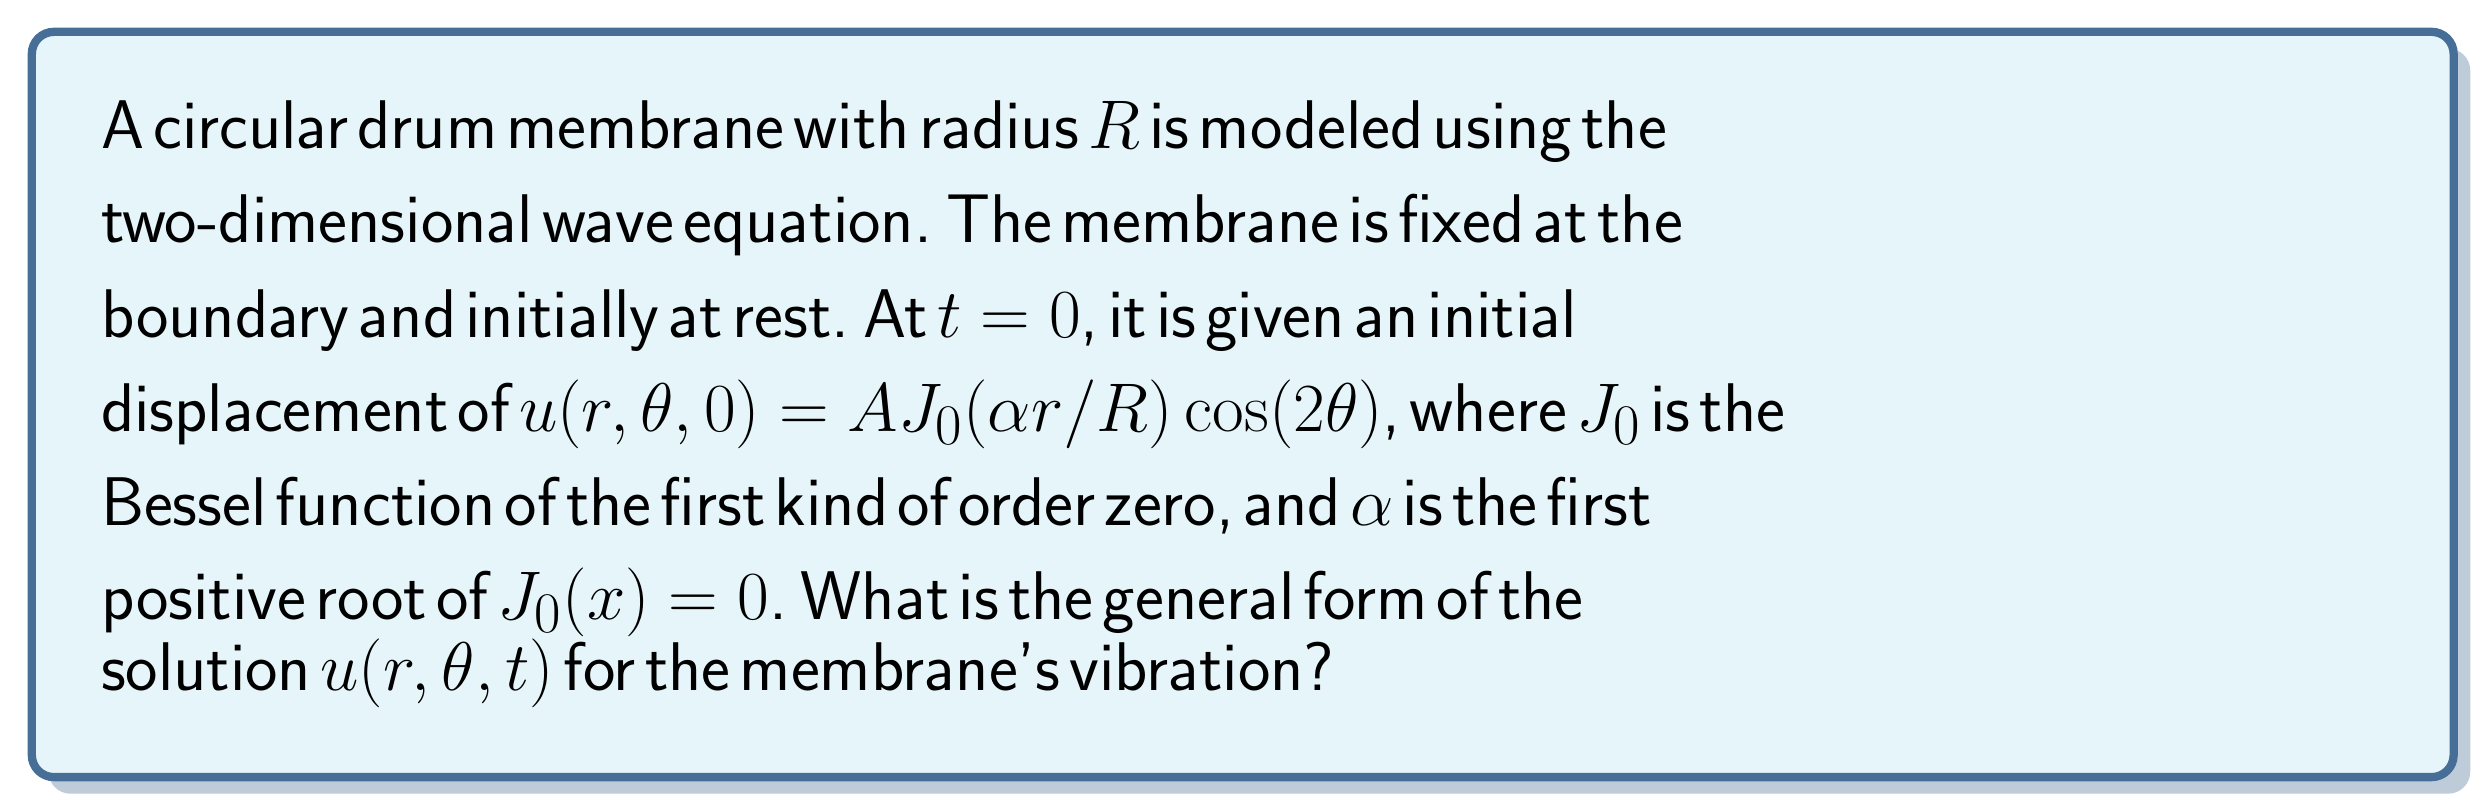
\begin{tikzpicture}
    % Define colors
    \definecolor{bordercolor}{RGB}{70,110,150}
    \definecolor{fillcolor}{RGB}{230,245,250}
    
    % Draw the rounded rectangle box
    \node[
        rectangle,
        rounded corners=8pt,
        drop shadow={shadow xshift=6pt, shadow yshift=-6pt, fill=bordercolor, opacity=0.35},
        draw=bordercolor,
        line width=3pt,
        fill=fillcolor,
        text width=29cm,
        align=left,
        inner sep=25pt
    ] at (0,0) {
        \sffamily\fontsize{28}{34}\selectfont
        A circular drum membrane with radius $R$ is modeled using the\\
        two-dimensional wave equation. The membrane is fixed at the\\
        boundary and initially at rest. At $t = 0$, it is given an initial\\
        displacement of $u(r,\theta,0) = A J_0(\alpha r/R)\cos(2\theta)$, where $J_0$ is the\\
        Bessel function of the first kind of order zero, and $\alpha$ is the first\\
        positive root of $J_0(x)=0$. What is the general form of the\\
        solution $u(r,\theta,t)$ for the membrane's vibration?
    };
    
\end{tikzpicture}

\end{document}
